% Options for packages loaded elsewhere
\PassOptionsToPackage{unicode}{hyperref}
\PassOptionsToPackage{hyphens}{url}
\PassOptionsToPackage{dvipsnames,svgnames,x11names}{xcolor}
%
\documentclass[
  letterpaper,
  DIV=11,
  numbers=noendperiod]{scrartcl}

\usepackage{amsmath,amssymb}
\usepackage{iftex}
\ifPDFTeX
  \usepackage[T1]{fontenc}
  \usepackage[utf8]{inputenc}
  \usepackage{textcomp} % provide euro and other symbols
\else % if luatex or xetex
  \usepackage{unicode-math}
  \defaultfontfeatures{Scale=MatchLowercase}
  \defaultfontfeatures[\rmfamily]{Ligatures=TeX,Scale=1}
\fi
\usepackage{lmodern}
\ifPDFTeX\else  
    % xetex/luatex font selection
\fi
% Use upquote if available, for straight quotes in verbatim environments
\IfFileExists{upquote.sty}{\usepackage{upquote}}{}
\IfFileExists{microtype.sty}{% use microtype if available
  \usepackage[]{microtype}
  \UseMicrotypeSet[protrusion]{basicmath} % disable protrusion for tt fonts
}{}
\makeatletter
\@ifundefined{KOMAClassName}{% if non-KOMA class
  \IfFileExists{parskip.sty}{%
    \usepackage{parskip}
  }{% else
    \setlength{\parindent}{0pt}
    \setlength{\parskip}{6pt plus 2pt minus 1pt}}
}{% if KOMA class
  \KOMAoptions{parskip=half}}
\makeatother
\usepackage{xcolor}
\setlength{\emergencystretch}{3em} % prevent overfull lines
\setcounter{secnumdepth}{5}
% Make \paragraph and \subparagraph free-standing
\ifx\paragraph\undefined\else
  \let\oldparagraph\paragraph
  \renewcommand{\paragraph}[1]{\oldparagraph{#1}\mbox{}}
\fi
\ifx\subparagraph\undefined\else
  \let\oldsubparagraph\subparagraph
  \renewcommand{\subparagraph}[1]{\oldsubparagraph{#1}\mbox{}}
\fi


\providecommand{\tightlist}{%
  \setlength{\itemsep}{0pt}\setlength{\parskip}{0pt}}\usepackage{longtable,booktabs,array}
\usepackage{calc} % for calculating minipage widths
% Correct order of tables after \paragraph or \subparagraph
\usepackage{etoolbox}
\makeatletter
\patchcmd\longtable{\par}{\if@noskipsec\mbox{}\fi\par}{}{}
\makeatother
% Allow footnotes in longtable head/foot
\IfFileExists{footnotehyper.sty}{\usepackage{footnotehyper}}{\usepackage{footnote}}
\makesavenoteenv{longtable}
\usepackage{graphicx}
\makeatletter
\def\maxwidth{\ifdim\Gin@nat@width>\linewidth\linewidth\else\Gin@nat@width\fi}
\def\maxheight{\ifdim\Gin@nat@height>\textheight\textheight\else\Gin@nat@height\fi}
\makeatother
% Scale images if necessary, so that they will not overflow the page
% margins by default, and it is still possible to overwrite the defaults
% using explicit options in \includegraphics[width, height, ...]{}
\setkeys{Gin}{width=\maxwidth,height=\maxheight,keepaspectratio}
% Set default figure placement to htbp
\makeatletter
\def\fps@figure{htbp}
\makeatother
\newlength{\cslhangindent}
\setlength{\cslhangindent}{1.5em}
\newlength{\csllabelwidth}
\setlength{\csllabelwidth}{3em}
\newlength{\cslentryspacingunit} % times entry-spacing
\setlength{\cslentryspacingunit}{\parskip}
\newenvironment{CSLReferences}[2] % #1 hanging-ident, #2 entry spacing
 {% don't indent paragraphs
  \setlength{\parindent}{0pt}
  % turn on hanging indent if param 1 is 1
  \ifodd #1
  \let\oldpar\par
  \def\par{\hangindent=\cslhangindent\oldpar}
  \fi
  % set entry spacing
  \setlength{\parskip}{#2\cslentryspacingunit}
 }%
 {}
\usepackage{calc}
\newcommand{\CSLBlock}[1]{#1\hfill\break}
\newcommand{\CSLLeftMargin}[1]{\parbox[t]{\csllabelwidth}{#1}}
\newcommand{\CSLRightInline}[1]{\parbox[t]{\linewidth - \csllabelwidth}{#1}\break}
\newcommand{\CSLIndent}[1]{\hspace{\cslhangindent}#1}

\usepackage{booktabs}
\usepackage{longtable}
\usepackage{array}
\usepackage{multirow}
\usepackage{wrapfig}
\usepackage{float}
\usepackage{colortbl}
\usepackage{pdflscape}
\usepackage{tabu}
\usepackage{threeparttable}
\usepackage{threeparttablex}
\usepackage[normalem]{ulem}
\usepackage{makecell}
\usepackage{xcolor}
\addtokomafont{disposition}{\rmfamily}
\KOMAoption{captions}{tableheading}
\makeatletter
\makeatother
\makeatletter
\makeatother
\makeatletter
\@ifpackageloaded{caption}{}{\usepackage{caption}}
\AtBeginDocument{%
\ifdefined\contentsname
  \renewcommand*\contentsname{Table of contents}
\else
  \newcommand\contentsname{Table of contents}
\fi
\ifdefined\listfigurename
  \renewcommand*\listfigurename{List of Figures}
\else
  \newcommand\listfigurename{List of Figures}
\fi
\ifdefined\listtablename
  \renewcommand*\listtablename{List of Tables}
\else
  \newcommand\listtablename{List of Tables}
\fi
\ifdefined\figurename
  \renewcommand*\figurename{Figure}
\else
  \newcommand\figurename{Figure}
\fi
\ifdefined\tablename
  \renewcommand*\tablename{Table}
\else
  \newcommand\tablename{Table}
\fi
}
\@ifpackageloaded{float}{}{\usepackage{float}}
\floatstyle{ruled}
\@ifundefined{c@chapter}{\newfloat{codelisting}{h}{lop}}{\newfloat{codelisting}{h}{lop}[chapter]}
\floatname{codelisting}{Listing}
\newcommand*\listoflistings{\listof{codelisting}{List of Listings}}
\makeatother
\makeatletter
\@ifpackageloaded{caption}{}{\usepackage{caption}}
\@ifpackageloaded{subcaption}{}{\usepackage{subcaption}}
\makeatother
\makeatletter
\@ifpackageloaded{tcolorbox}{}{\usepackage[skins,breakable]{tcolorbox}}
\makeatother
\makeatletter
\@ifundefined{shadecolor}{\definecolor{shadecolor}{rgb}{.97, .97, .97}}
\makeatother
\makeatletter
\makeatother
\makeatletter
\makeatother
\ifLuaTeX
  \usepackage{selnolig}  % disable illegal ligatures
\fi
\IfFileExists{bookmark.sty}{\usepackage{bookmark}}{\usepackage{hyperref}}
\IfFileExists{xurl.sty}{\usepackage{xurl}}{} % add URL line breaks if available
\urlstyle{same} % disable monospaced font for URLs
\hypersetup{
  pdftitle={Finding suitable weather indices for novel fisheries index insurance using machine learning},
  pdfauthor={Nathaniel Grimes},
  pdfkeywords={Index Insurance, Fisheries, Machine Learning},
  colorlinks=true,
  linkcolor={blue},
  filecolor={Maroon},
  citecolor={Blue},
  urlcolor={Blue},
  pdfcreator={LaTeX via pandoc}}

\title{Finding suitable weather indices for novel fisheries index
insurance using machine learning}
\usepackage{etoolbox}
\makeatletter
\providecommand{\subtitle}[1]{% add subtitle to \maketitle
  \apptocmd{\@title}{\par {\large #1 \par}}{}{}
}
\makeatother
\subtitle{Working Paper not for Distribution}
\author{Nathaniel Grimes}
\date{2024-10-14}

\begin{document}
\maketitle
\begin{abstract}
Index insurance is a financial tool gaining traction for application in
fisheries. It will cover fishers losses under extreme weather events
that impact fishery productivity. This is the first assessment to
determine the feasibility of such programs and whether suitable indices
exist. Catch and revenue data from 74 California fisheries are matched
to 20 environmental variables using three prediction models: linear
regression, LASSO regression, and random forests. The models are used to
calculate the utility improvements of index insurance for fishers.
Random forests provide the most significant improvements in utility,
increasing fisher welfare by 14\%. The results suggest that index
insurance can improve fisher welfare, but the extent of success is not
consistent across all fisheries. Specifically tailored insurance
contracts must be created for each fishery using the best available data
and models
\end{abstract}
\ifdefined\Shaded\renewenvironment{Shaded}{\begin{tcolorbox}[breakable, borderline west={3pt}{0pt}{shadecolor}, boxrule=0pt, enhanced, frame hidden, interior hidden, sharp corners]}{\end{tcolorbox}}\fi

\renewcommand*\contentsname{Table of contents}
{
\hypersetup{linkcolor=}
\setcounter{tocdepth}{3}
\tableofcontents
}
\hypertarget{introduction}{%
\section{Introduction}\label{introduction}}

Predicting fishery output from weather variables is notoriously
difficult. It is widely established that climate and weather affect
fishing populations (Lehodey \emph{et al.} 2006), but most stock
assessment models use little to no year to year environmental data
(Privitera-Johnson and Punt 2020). Variations in environmental
conditions are now the leading cause of fishery closures and disaster
relief payouts in the United States (Bellquist \emph{et al.} 2021).
Disaster declarations are becoming more frequent straining a slow,
inequitable system (Holland and Leonard 2020; Jardine \emph{et al.}
2020). Calls for new financial tools to alleviate fisher income shocks
have grown (Mumford \emph{et al.} 2009; Sethi 2010).

Index insurance has risen as a prime candidate to protect fishing
communities during disasters (Watson \emph{et al.} 2023). Index
insurance is a financial product that pays out when an independently
verified index, such as rainfall or temperature, falls below a
predetermined threshold. The index is chosen to be highly correlated
with the asset being insured. However, it is difficult to establish
clear, concise weather impacts on fishery productivity. The biological
dynamics of the system can lead to lower stock health persisting for
years after a negative shock (\textbf{Hilborn2003?}). Individual
fisheries can cover enormous areas in ocean basins. The expansive
spatial coverage of fisheries makes it unclear where and how much
specific weather variables impact biological abundance. In addition, if
weather impacts have been observed, they are most likely highly
non-linear adding further complexity. The greatest impediment to the
development of fishery insurance policies is reconciling these
challenges to find suitable indices that can predict fishery
productivity (Watson \emph{et al.} 2023).

Recent expansions in oceanic remote sensing has led to a plethora of new
environmental indices that could be used to predict fishery
productivity. Fishery data collection continues to improve with better
reporting systems with longer and more detailed catch histories. This
study aims to leverage these improved data sources to create suitable
indices for fisheries index insurance using machine learning.

The difficulty in modelling fishery productivity with environmental
indices leads to basis risk. Formally, basis risk is the probability
that policyholders experience a harmful shock to their income, but the
index does not trigger. Basis risk lowers demand for index insurance and
remains a significant roadblock in setting up new programs
(Binswanger-Mkhize 2012; Clarke 2016; Clement \emph{et al.} 2018).

It is impossible to completely eliminate basis risk, and there exists a
wide range in exisiting agriculture products. Well designed policies can
capture up to 90\% of the income variation as shown in Kenyan pasture
grazing indices (Jensen \emph{et al.} 2019). Abysmal correlations are
prevalent in the Rainfall Index Insurance for Pasture, Rangeland, and
Forage (RI-PRF) program where correlations as low as 0.071 exist in
California, which leads to 46\% additional points of basis risk (Keller
and Saitone 2022). The program has a 26\% probability of not paying out
when damages are suffered in Nebraska and Kansas (Yu \emph{et al.}
2019). Subsidies covering up to 60\% of ranchers paid premiums are
needed to stimulate demand in the RI-PRF program (Goodrich \emph{et al.}
2019).

Contract design can mitigate basis risk through providing more options
so that individuals can better select policies that protect them.
Policyholders choose lower trigger levels when correlations between
between index and asset are low (Lichtenberg and Iglesias 2022). Lower
trigger levels correspond to protection against more catastrophic
shocks. Increased contract flexibility reduces basis risk by only small
amounts. Yu \emph{et al.} (2019) found that more flexible contracts
could account for only 5-9\% of basis risk. Farms in Kansas closer to
weather stations had better predictive impacts of rain on yield (Yu
\emph{et al.} 2019).

Designing indices with stronger correlations to fishery losses is the
most effective way to reduce basis risk (Jensen \emph{et al.} 2019).
Agricultural researchers continually seek new methods and data sources
to improve the correlation between loss and weather variables. Quantile
regressions improve Kazak wheat farmers utility between 0.1-22\% over
linear models depending on the underlying measure of utility (Conradt
\emph{et al.} 2015). Remote sensing variables leveraging the latest
satellite data on vegetative cover and rainfall provide better coverage
than county wide averages (Dalhaus and Finger 2016; Valverde-Arias
\emph{et al.} 2020).

Machine learning has exploded as a new method to define better indices
in agriculture index insurance (Feng \emph{et al.} 2019; Cesarini
\emph{et al.} 2021; Schmidt \emph{et al.} 2022; Chen \emph{et al.}
2024). Machine learning models excel in index insurance because
indemnity contracts only need predictive relationships. Whereas, fishery
stock assessments build complex models with biological foundations to
accurately inform management of future fish stocks, index insurance can
look retroactively at data to uncover relationships and test out of
sample predictive quality. Machine learning may be necessary in
fisheries index insurance to uncover any valuable relationships between
weather and productivity.

The application of machine learning is growing in fisheries as
researchers explore data questions beyond formal stock assessments.
Ensemble models built through combinations of random forests, boosted
trees, and dynamic linear models improved Bristol Bay sockeye salmon
forecasts by 15\% compared to a standard lagged regression model (Ovando
\emph{et al.} 2022). Environmental variables of importance to groundfish
populations in Alaska were uncovered using single index varying
coefficient models regularized with LASSO (Correia 2021). Random Forests
models better predict fish catch in Indonesia than traditional linear
models (Rahman \emph{et al.} 2022). The expected non-linear interactions
of weather and fishery productivity merit the use of machine learning in
fisheries.

This study will provide the first comprehensive examination of the
necessary features of weather indices for fisheries index insurance. We
contribute to the growing ocean adaption and blue finance literature.
While our intent is to improve fisher welfare with a new financial
program, we also expand the assessment of which weather variables have
predictive performance in highly productive upwelling ecosystems.

The rest of the paper is structured as follows. Section~\ref{sec-model}
describes the insurance model tested in this study.
Section~\ref{sec-data} describes the data collection, transformations,
and sources. Fisheries data comes from newly open-access sources
provided by the California Department of Fish and Wildlife.
Section~\ref{sec-methods} describes the algorithms used to predict
fishery productivity and evaluate the utility of index insurance.
Section~\ref{sec-results} presents the welfare results as well as
extracting which variables contribute to the prediction models to infer
more interpretable results for fishers. Section~\ref{sec-discussion}
discusses the results and implications for the future of fisheries index
insurance.

\hypertarget{sec-model}{%
\section{Insurance Model}\label{sec-model}}

Insurance contracts are specified by calculating payout functions
(\(I(\omega)\)) based on independently measured weather variables.
Neural networks have been used to provide non-linear payoff schedules
that better reduce basis risk (Chen \emph{et al.} 2024). While it has
been shown that linear payoff functions inherently lead to basis risk
and therefore lower demand (Clarke 2016; Jensen \emph{et al.} 2016), we
maintain their use to preserve measures of interpretability that are
clearer for a first analysis of fishery index insurance.

Payouts will be issued when prediction models predict negative
deviations from the long run average. The three prediction models
(\(k\in\{\text{LR,LA,RF}\}\) are a linear regression (\(\text{LR}\)), a
LASSO regression (\(\text{LA}\)), and a random forest (\(\text{RF}\)).

\begin{equation}\protect\hypertarget{eq-payout}{}{
I(\omega)=\max(0,(\bar{\pi}-\hat\pi_t^k(\omega)) \cdot l)
}\label{eq-payout}\end{equation}

Where \(k\) is the prediction model, \(l\) is the level of coverage,
\(\hat\pi_t^k(w)\) is the predicted fishing variable from \(\omega\)
weather variables, and \(\bar{\pi}\) the long run average of the fishing
variable. The premium \(\rho\) is calculated as the expected value of
the payout function times the premium loading factor \(m\)
(Equation~\ref{eq-premium}).

\begin{equation}\protect\hypertarget{eq-premium}{}{
\rho(\omega)=\mathbb{E}[I(\omega)]m
}\label{eq-premium}\end{equation}

Utility measures offer the most insightful evaluation of index insurance
policies (Kenduiywo \emph{et al.} 2021). It captures value added for
policyholders, not just measures of payout frequency as other measures
of basis risk. Constant absolute risk aversion allows more consistent
comparison for different levels of wealth. Fishing variables may vary
extensively from fishery to fishery. We normalize utility by dividing
all measured payouts and fishing variables by the maximum observed
value. Expected utility for a given fishery is the average utility over
all years in the sample for any variable of interest \(\pi_t\). Fishers
are allowed to choose insurance coverage levels \(l\) to ensure feasible
contracts.

\begin{equation}\protect\hypertarget{eq-utility}{}{
\begin{aligned}
\mathbb{E}[U_{b}]&=\frac{1}{n}\sum_{t}^{T}\frac{1-e^{-a\pi_t}}{a} &\text{No Insurance}\\
\mathbb{E}[U_{i}]&=\max_{l}\frac{1}{n}\sum_{t}^{T}\frac{1-e^{(-a(\pi_t+I(\omega,l)-\rho(w))}}{a} &\text{Insurance}\\
U_{r}&=\frac{\mathbb{E}[U_i]-\mathbb{E}[U_b]}{\mathbb{E}[U_b]}\cdot100 &\text{Percent Change in Utility}\\
\end{aligned}
}\label{eq-utility}\end{equation}

We will compare the percent change in fisher utility with insurance
(\(U_i\)) versus without insurance (\(U_{b}\)) for each prediction
method. The variable of interest \(\pi_t\), will be fishing revenue,
landings, and revenue per fisher to test what measures of fishery
productivity are most suitable for index insurance.

No data on fishery insurance suppliers exists to create a market
equilibrium. We iteratively vary the premium loading \(m\in[1,2]\) to
create a range of coverage values fishers will be willing to pay for a
given \(m\). Then, the amount of coverage purchased times the premium
loading factor approximately equals the expected revenue an insurance
company would receive. Insurance companies could then examine their own
administrative and legal costs to determine whether the feasible
contract is profitable.

\hypertarget{sec-data}{%
\section{Data}\label{sec-data}}

This study attempts to cover breadth, not depth in possible indices.
Each fishery has unique ecological characteristics that interact with
environmental variables in different and non-linear ways. By studying a
wide collection of fisheries and environmental variables we can uncover
the potential feasibility of index insurance for fisheries holistically,
and then further refine measures with ecologically sound models in
future applications.

\hypertarget{fishery-data}{%
\subsection{Fishery Data}\label{fishery-data}}

Landings revenue, and participation data comes from the West Coast Fish
data package (Free \emph{et al.} 2022). It is a reconstruction of
California Fish and Wildlife Department catch data combined with PacFin
receipts for Washington and Oregon. The last three years of data are
updated from the CDFW Marine Fisheries Data Explorer (MFDE). Names are
matched to each species within the West Coast Fish data package.

We select California fisheries with a minimum of 30 years of
consecutive, non-confidential catch records at both the state and
port-complex level. Unclassified catch records are dropped i.e.~``Other
Sharks'' and similar categories. Fisheries with an average revenue from
2010-2019 greater than \$100,000 at the state and \$75,000 at
port-complex level are analyzed. Twenty four fisheries at the state
level and 50 fisheries at the port complex level meet these criteria.
These fisheries contain the most economically important fisheries in
California and their mean values are shown in Table~\ref{tbl-fish-sum}
and at the port complex in Table~\ref{tbl-fish-port-sum}.

Fisheries have complex spatial dynamics. Agriculture has clear,
quantifiable impacts of weather in grids that are well suited for index
insurance. Drought on a single farm directly leads to crop loss for that
farm. Whether there is sufficient spatial coverage to identify impacts
down to an individual farm remains a challenge in agriculture (Dalhaus
and Finger 2016; Leppert \emph{et al.} 2021; Stigler and Lobell 2024).
Fish and fishers can move thousand of miles in a given year, thus more
consideration must be given to the location of weather impacts in
fisheries. We spatially refine catch histories using the California CDFW
fishing blocks records from the MFDE Data Explorer. Summarized catch
histories of all landed fish within each block provide an average
representation of effort for a given fishery. Spatial catch history is
measured at both the state and port-complex level. The spatial location
refines the location of environmental variables. Local weather is more
likely to affect fishery productivity and catch than observations
thousands of miles away.

\hypertarget{environmental-data}{%
\subsection{Environmental Data}\label{environmental-data}}

Fisheries are highly sensitive to marine heatwaves and water
temperature. Sea surface temperature is a natural variable to first
consider in fisheries index insurance. Sea surface temperature data
comes from the NOAA DHW data set that provides 5-km resolution of
monthly temperature from 1985 to 2023. The 5-km grids are averaged
within the nearest California fishing block to provide an annual time
series of temperature for each fishery. Temperature is lagged from 1 to
3 years prior to account for residual impacts that carry over due to
fishery biological dynamics.

Upwelling provides vital nutrients to stimulate primary productivity.
The coast of California is a highly productive ecosystem due to its
patterns of upwelling (Chelton \emph{et al.} 1982; Huyer 1983). We
capture upwelling through monthly observations of Coastal Upwelling
Transport Index (CUTI) and Biological Effective Upwelling Transport
Idnex (BEUTI). Both indices create measures of vertical movement in the
mixed layer at 1 degree latitude intervals extending 75 km along the
entire US West Coast (Jacox \emph{et al.} 2018). The closest layer to
the surface was used in this analysis as the correlation between surface
index values and deeper index values are high. CUTI examines the
physical measures of wind, ekman transport, and cross-shore geostrophic
transport to indicate the strength of upwelling in a given month. BEUTI
adds nitrate concentration in its calculation to capture more biological
effects of upwelling. Fishing blocks are matched to the nearest 1 degree
latitude interval to provide a monthly time series of upwelling for each
fishery. Seasonal strengths of upwelling are captured by averaging CUTI
and BEUTI within each quarter of the year. Spring upwelling in early
March and April are especially important to a wide array of fish
species. Yearly average and amplitude values (the difference between
minimum observed upwelling and maximum) are also calculated. These
indices are the most temporally limited datasets in this analysis, only
extending from 1988 to 2023.

The Habitat Compression Index measures the area extent of water below
average temperatures thresholds along the US West Coast (Schroeder
\emph{et al.} 2022). Habitat compression is a measure of the spatial
extent of cold water habitats that are important for fish species. The
index is broken down into four distinct oceangraphic regions ranging
from 3.5 degrees to 5.5 degrees lattitude in size with coverage out to
150 km offshore. We use the cumulative habitat compression index that
sums the index value in each month to provide a yearly time series of
habitat compression for each fishery. The cumulative index showed
stronger correlations with biological productivity measures than monthly
measures (Schroeder \emph{et al.} 2022)

The final environmental variables are the Pacific Decadal Oscillation
(PDO) and the El Nino Southern Oscillation (ENSO). Both indices are well
known to affect marine ecosystems and fisheries. Both indices are
averaged over a given year. PDO data is taken from the PDO ERSST V5, and
ENSO data is taken from the multivariate ENSO Index Version 2 (MEI.v2).

Summary statistics for the environmental data are presented in
Table~\ref{tbl-env-sum}. In total, 74 fisheries with 35 years of catch
data and 20 weather variables are spatially matched with annual coverage
from 1988 to 2023.

\hypertarget{sec-methods}{%
\section{Methods}\label{sec-methods}}

We use three models to predict yearly fishing revenue, landings, and
catch per fisher at state and port-complex levels. Linear models are
used as the base model given its ubiquitous use in index insurance
policies. We compare utility improvements with the adoption of more
robust LASSO regression and random forest models.

In all class of models, the final utility maximization choice of
coverage leverage is found through a box constrained quasi-Newton Method
using the optim function in R. Choices are constrained to be
non-negative. Premium schedules are found by the model output below the
trigger values in Equation~\ref{eq-payout} and then averaged over the
total fishery data.

\hypertarget{linear-models}{%
\subsection{Linear Models}\label{linear-models}}

Perfect regression coefficients mimic the optimal choice of scale in
index insurance contracts (\textbf{Mahul1999?}). Combined with the ease
of implementation, linear models on single weather indices are the most
common design choice for index insurance policies. They offer a basic
starting place to consider the viability of fishery index insurance.

Yearly aggregated fishing variables are regressed on each environmental
variable individually. Weather variables are spatially matched to the
location of catch. We perform a 10 fold cross validation method to
determine the best individual weather variable based on root mean square
error (RMSE). To preserve the time series element of the data, we used a
rolling split to partition the training and testing data. For example,
the first fold contains the first 70\% of data as training (1988-2011),
and the last 30\% as testing (2013-2023). The final date of the training
set is extended in each fold until the year 2020 to create 10 folds.
Models with the lowest average RMSE are selected and trained on the full
set before being passed to the utility optimization procedure in
Equation~\ref{eq-utility}.

\hypertarget{lasso-regression}{%
\subsection{LASSO Regression}\label{lasso-regression}}

Least Absolute Shrinkage and Selection Operator (LASSO) regression is a
popular regularization technique to assist model selection. It attempts
to minimize the residual sum of squared errors through Ordinary Least
Squares (OLS), but adds a penalty constraint on the absolute sum of
selected coefficient values (Equation~\ref{eq-lasso}).

\begin{equation}\protect\hypertarget{eq-lasso}{}{
\hat{\beta}^{lasso}=\arg\min_{\beta}\left\{\sum_{i=1}^{n}(y_i-\beta_0-\sum_{j=1}^{p}\omega_{ij}\beta_j)^2+\lambda\sum_{j=1}^{p}|\beta_j|\right\}
}\label{eq-lasso}\end{equation}

Where, \(y_i\) is our fishing variable, \(\beta\) the regression
coefficients, \(n\), the number of observations, \(p\) the number of
predictors, and \(\omega\) the total collection of weather variables.
The \(\lambda\) is the penalty term that controls the amount of
shrinkage. Models are trained using the \texttt{glmnet} package in R.
The LASSO regression model is trained on 200 bootstrapped samples of the
training data. The optimal \(\lambda\) is selected through a grid search
method that selects the minimum RMSE. This choice is to ensure the most
parsimonious model that still captures the most important weather
variables. LASSO is particularly well suited for this research design as
the absolute value of the penalty term shrinks coefficients to zero.
Overfitting is a concern with so few observations in the initial
training set; the shrinkage towards zero will help minimize this bias by
reducing the parameter space.

\hypertarget{random-forests}{%
\subsection{Random Forests}\label{random-forests}}

While LASSO offers us the ability to simultaneously explore a wide
collection of weather variables including lagged effects, it remains
linear in its predictions. Random Forests are tree-based ensemble models
that capture non-linear interactions through recursive partitioning.
They are less sensitive to over fitting through the aggregation of many
trees.

We tune two hyperparameters to create the best performing random forest
for each fishery: The number of variables to consider at each split and
the minimum number of observations in a leaf node. We use a grid search
method to find the best hyperparameters based on RMSE through the year
based cross validation method presented in the linear models. The final
model is trained on the full dataset and passed to the utility
optimization procedure in Equation~\ref{eq-utility}.

\hypertarget{weather-variables-of-importance}{%
\subsection{Weather variables of
importance}\label{weather-variables-of-importance}}

Machine learning algorithms are inherently ``black boxes'' that
sacrifice interpreability for predictive accuracy. Fishers will be less
likely to purchase complicated products that do not correspond to their
experiences. Extracting the relative contribution of weather variables
will assist translating products to fishers. Additionally, it can help
ground-truth the chosen variables with previous biological modelling.

The cross-validation in the linear models provides a simple weather
variable comparison. We calculate the frequency a given weather variable
is chosen as the best performing linear model.

We use \texttt{vip} package in R to extract importance measures for both
the LASSO and random forests \footnote{Nathan note: I need to read more
  exactly how this package will extract between permutations or variance
  measures}. Feature extraction will occur for each fishery product, and
the importance of each will be normalized then aggregated in order to
compare all features.

\hypertarget{sec-results}{%
\section{Results}\label{sec-results}}

Index insurance can improve fisher utility even with univariate linear
models, but the extent of success is not consistent across all
fisheries. At actuarially fair premiums, \(m=1\), the average utility
improvement for fishers with linear models is approximately 2\% at the
state level of all fishing dependent variables
(Table~\ref{tbl-utility-state}). LASSO increases the utility gains of
index insurance through better performing indices. The improvements
slightly depend on the fishery dependent variable. Targeting fishing
revenues provides more than 1\% additional gains in utility over
landings. Revenues may be more difficult to predict as they incorporate
external market factors such as price and demand, but revenues more
closely match the financial interests of fishers.

Random forests provide the most significant improvements in utility. The
ability to capture the non-linear interactions of weather variables with
fishery productivity provides much more accurate trigger states that
more closely align with lost value. All three fishery dependent trigger
variables with random forest models improved fisher utility by 14\%.

\hypertarget{tbl-utility-state}{}
\begin{table}
\caption{\label{tbl-utility-state}Average relative percent improvement in utility for 24 fisheries at the
state level. Standard deviations in utilty are included in parathesis.
Fishers }\tabularnewline

\centering
\begin{tabular}{llll}
\toprule
 & Landings & Revenue & Revenue per Fisher\\
\midrule
Linear & 2.4\%
(2.7) & 2.1\%
(2.8) & 2.4\%
(2.7)\\
LASSO & 6.3\%
(6.4) & 7.3\%
(8.3) & 8\%
(6.2)\\
Random Forest & 13.9\%
(10.8) & 14.7\%
(10) & 14\%
(8.6)\\
\bottomrule
\end{tabular}
\end{table}

The range of responses varies for each fishery. Inherent volatility and
model performance drive the differences. Chinook Salmon saw the largest
gain in utility out of all fisheries with a random forest model
triggered on revenues (Figure~\ref{fig-cali-rev}). Random forests always
led to utility improvements, whereas LASSO and linear models maintained
exorbitant basis risk compelling fishers to choose no insurance in
Pacific Bonito, Cabezon, and California Sheephead

\begin{figure}

{\centering 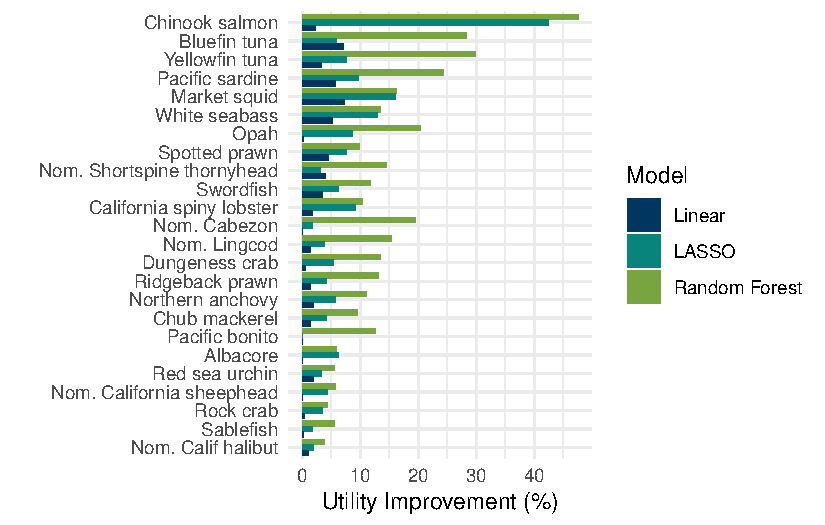
\includegraphics{ibi-ml_files/figure-pdf/fig-cali-rev-1.pdf}

}

\caption{\label{fig-cali-rev}Utility improvements for California
fisheries with index insurance with a revenue trigger. Random Forest
models (green) provide the greatest utility imporvement relative to no
insurnace. LASSO (teal) generally out performs linear models (blue).}

\end{figure}

Different triggers maintain the same magntiude of improvements, but
benefit to specific fisheries can change (Figure~\ref{fig-cali-mt}).

\begin{figure}

{\centering 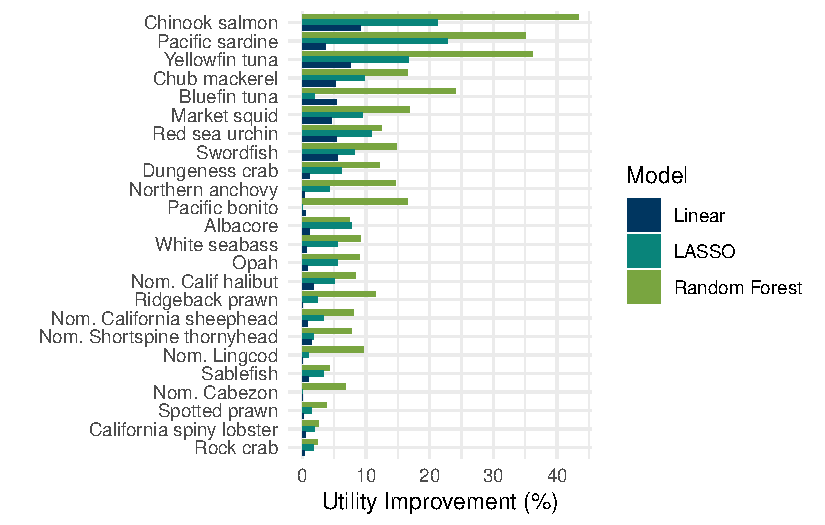
\includegraphics{ibi-ml_files/figure-pdf/fig-cali-mt-1.pdf}

}

\caption{\label{fig-cali-mt}Utility improvements for California
fisheries with index insurance with a landings trigger. Random Forest
models (green) provide the greatest utility imporvement relative to no
insurnace. LASSO (teal) generally out performs linear models (blue).}

\end{figure}

Results are consistent when looking at the port-complex level, though
LASSO and random forest have 2\% less utility improvements than at the
state level (Table~\ref{tbl-utility-port}). Large discrepncies can exist
between port-complexes for the same insurance policies. For example, an
insurance contract for Chinook Salmon based on metric tons at the
California state level improved utility by 21\%. However, different port
complexes choose different levels of coverage (\textbf{?@tbl-chnk}).
Eureka was the most extreme difference by opting for no insurance. The
weather variability was not captured sufficiently by the LASSO model in
Eureka and could not provide enough smoothing to incentivize fishers to
purchase insurance. This observation emphasizes the benefit of creating
policies at the port-complex level as the local variations capture basis
risk exposure to each unique community \footnote{Nathan note: Should
  compare the eureka port-complex data with the cali lasso model to see
  if they would want insurance with that. Kind of a robustness check}.

\hypertarget{tbl-utility-port}{}
\begin{table}
\caption{\label{tbl-utility-port}Average relative percent improvement in utility for 50 fisheries at the
port complex level. }\tabularnewline

\centering
\begin{tabular}{llll}
\toprule
 & Landings & Revenue & Revenue per Fisher\\
\midrule
Linear & 1.9\%
(2.6) & 1.9\%
(3.4) & 2.7\%
(3.9)\\
LASSO & 4.9\%
(4.8) & 6\%
(5) & 6.7\%
(5)\\
Random Forest & 11.8\%
(6.9) & 12.8\%
(6.2) & 12.5\%
(6.9)\\
\bottomrule
\end{tabular}
\end{table}

\hypertarget{sec-discussion}{%
\section{Discussion}\label{sec-discussion}}

\textbf{Remaining things do to}

\begin{itemize}
\item
  Variable importance
\item
  Feasibility of interprebable models
\item
  Alter m off actuarilly fair
\item
  Change utility models
\item
  Make a payout frequency table
\item
  Show the income smoothing effect as a distribution
\end{itemize}

\hypertarget{appendix}{%
\section{Appendix}\label{appendix}}

\hypertarget{tbl-fish-sum}{}
\begin{table}
\caption{\label{tbl-fish-sum}Summary statistics of catch from 1988-2023 for California fisheries. }\tabularnewline

\centering
\resizebox{\ifdim\width>\linewidth\linewidth\else\width\fi}{!}{
\begin{tabular}{lrrlrrrrr}
\toprule
\multicolumn{1}{c}{ } & \multicolumn{2}{c}{Landings (mt)} & \multicolumn{2}{c}{Revenue (USD)} & \multicolumn{2}{c}{MT per Fisher} & \multicolumn{2}{c}{Number of Fishers} \\
\cmidrule(l{3pt}r{3pt}){2-3} \cmidrule(l{3pt}r{3pt}){4-5} \cmidrule(l{3pt}r{3pt}){6-7} \cmidrule(l{3pt}r{3pt}){8-9}
Species & Mean & SD & Mean & SD & Mean & SD & Mean & SD\\
\midrule
Albacore & 2055.4 & 2646.5 & \$3,574,984 & 4051538.3 & 5.3 & 3.1 & 305.5 & 307.7\\
Bluefin tuna & 760.5 & 1131.1 & \$1,118,896 & 1137192.5 & 9.3 & 12.1 & 76.3 & 46.1\\
California spiny lobster & 314.6 & 69.6 & \$7,752,729 & 5402314.5 & 1.7 & 0.6 & 202.0 & 39.8\\
Chinook salmon & 1576.1 & 1291.7 & \$10,383,616 & 7643140.9 & 1.5 & 1.1 & 1146.6 & 1022.2\\
Chub mackerel & 11304.3 & 10208.0 & \$1,944,342 & 1709450.2 & 80.2 & 59.5 & 133.9 & 78.6\\
\addlinespace
Dungeness crab & 5712.8 & 3334.7 & \$29,115,960 & 23070113.4 & 11.6 & 7.9 & 534.5 & 121.7\\
Market squid & 51363.6 & 34634.6 & \$27,517,541 & 24057582.4 & 462.1 & 289.5 & 109.4 & 23.4\\
Nom. Cabezon & 35.3 & 38.7 & \$306,669 & 321874.4 & 0.2 & 0.1 & 199.0 & 115.1\\
Nom. Calif halibut & 374.6 & 140.9 & \$2,605,362 & 873979.0 & 0.9 & 0.3 & 427.1 & 87.8\\
Nom. California sheephead & 46.7 & 38.8 & \$342,986 & 231782.3 & 0.4 & 0.2 & 134.1 & 88.5\\
\addlinespace
Nom. Lingcod & 359.0 & 421.0 & \$388,778 & 276453.1 & 0.4 & 0.3 & 675.4 & 374.0\\
Nom. Shortspine thornyhead & 56.4 & 70.0 & \$432,850 & 465662.0 & 0.5 & 0.6 & 116.2 & 35.6\\
Northern anchovy & 7696.1 & 10157.9 & \$860,871 & 643585.4 & 230.8 & 246.9 & 32.7 & 9.8\\
Opah & 102.4 & 100.0 & \$198,182 & 257248.5 & 2.5 & 3.6 & 71.0 & 46.8\\
Pacific bonito & 1090.7 & 1694.6 & \$544,835 & 886379.0 & 8.7 & 10.3 & 108.2 & 168.6\\
\addlinespace
Pacific sardine & 20665.4 & 22757.5 & \$2,574,205 & 2614838.8 & 309.1 & 325.9 & 53.3 & 21.0\\
Red sea urchin & 7947.2 & 6067.5 & \$11,443,321 & 7684762.0 & 32.7 & 12.7 & 231.1 & 139.5\\
Ridgeback prawn & 172.8 & 146.5 & \$634,305 & 473336.8 & 7.7 & 5.7 & 26.1 & 12.6\\
Rock crab & 620.2 & 146.3 & \$1,750,541 & 597289.3 & 3.6 & 1.2 & 180.7 & 47.4\\
Sablefish & 2753.2 & 1823.2 & \$5,759,976 & 2768043.7 & 10.4 & 6.9 & 269.6 & 70.3\\
\addlinespace
Spotted prawn & 153.1 & 76.1 & \$3,206,726 & 1989792.4 & 3.7 & 2.3 & 52.6 & 31.1\\
Swordfish & 808.3 & 554.7 & \$5,671,198 & 3401866.3 & 6.7 & 3.2 & 129.3 & 84.3\\
White seabass & 109.2 & 76.4 & \$635,876 & 429179.6 & 0.8 & 0.7 & 150.3 & 45.1\\
Yellowfin tuna & 8853.7 & 17403.5 & \$10,230,193 & 20959459.4 & 67.4 & 89.0 & 74.0 & 73.9\\
\bottomrule
\end{tabular}}
\end{table}

\hypertarget{tbl-fish-port-sum}{}
\begin{longtable}{llrrlrrrrr}
\caption{\label{tbl-fish-port-sum}Summary statistics of catch from 1988-2023 for California fisheries
split between species and port complex }\tabularnewline

\toprule
\multicolumn{2}{c}{ } & \multicolumn{2}{c}{Landings (mt)} & \multicolumn{2}{c}{Revenue (USD)} & \multicolumn{2}{c}{MT per Fisher} & \multicolumn{2}{c}{Number of Fishers} \\
\cmidrule(l{3pt}r{3pt}){3-4} \cmidrule(l{3pt}r{3pt}){5-6} \cmidrule(l{3pt}r{3pt}){7-8} \cmidrule(l{3pt}r{3pt}){9-10}
Species & Port & Mean & SD & Mean & SD & Mean & SD & Mean & SD\\
\midrule
 & Eureka & 355.0 & 377.4 & \$672,866 & 634894.5 & 5.4 & 3.4 & 62.2 & 58.9\\
\cmidrule{2-10}\nopagebreak
\multirow[t]{-2}{*}[1\dimexpr\aboverulesep+\belowrulesep+\cmidrulewidth]{\raggedright\arraybackslash Albacore} & San Francisco & 175.8 & 368.5 & \$322,734 & 639778.0 & 2.6 & 2.2 & 50.1 & 70.0\\
\cmidrule{1-10}\pagebreak[0]
Bluefin tuna & San Diego & 25.2 & 38.5 & \$163,167 & 334643.0 & 0.8 & 1.7 & 29.2 & 20.9\\
\cmidrule{1-10}\pagebreak[0]
 & Los Angeles & 47.2 & 36.2 & \$303,840 & 172626.8 & 0.7 & 0.3 & 64.0 & 25.9\\
\cmidrule{2-10}\nopagebreak
 & San Diego & 17.9 & 12.3 & \$117,380 & 51099.8 & 0.6 & 0.3 & 27.5 & 10.3\\
\cmidrule{2-10}\nopagebreak
 & San Francisco & 140.4 & 64.0 & \$1,053,595 & 721430.4 & 1.3 & 0.6 & 109.7 & 28.0\\
\cmidrule{2-10}\nopagebreak
\multirow[t]{-4}{*}[3\dimexpr\aboverulesep+\belowrulesep+\cmidrulewidth]{\raggedright\arraybackslash Nom. Calif halibut} & Santa Barbara & 97.9 & 44.4 & \$705,370 & 187398.0 & 1.1 & 0.3 & 87.1 & 22.3\\
\cmidrule{1-10}\pagebreak[0]
 & Bodega Bay & 329.6 & 309.3 & \$2,258,504 & 1989960.2 & 1.0 & 0.6 & 357.0 & 263.0\\
\cmidrule{2-10}\nopagebreak
 & Eureka & 103.6 & 178.4 & \$649,797 & 1000836.3 & 0.4 & 0.4 & 227.5 & 363.7\\
\cmidrule{2-10}\nopagebreak
 & Fort Bragg & 343.9 & 404.8 & \$2,320,248 & 2367832.3 & 1.1 & 1.4 & 357.0 & 263.0\\
\cmidrule{2-10}\nopagebreak
 & Monterey & 313.7 & 272.7 & \$1,896,626 & 1161527.4 & 0.9 & 0.6 & 354.0 & 201.8\\
\cmidrule{2-10}\nopagebreak
 & Morro Bay & 72.9 & 81.4 & \$493,105 & 515982.2 & 0.6 & 0.5 & 107.3 & 72.5\\
\cmidrule{2-10}\nopagebreak
\multirow[t]{-6}{*}[5\dimexpr\aboverulesep+\belowrulesep+\cmidrulewidth]{\raggedright\arraybackslash Chinook salmon} & San Francisco & 493.7 & 348.0 & \$3,339,479 & 2075261.9 & 1.2 & 0.8 & 434.7 & 265.1\\
\cmidrule{1-10}\pagebreak[0]
Chub mackerel & Los Angeles & 10320.4 & 9344.1 & \$1,782,814 & 1561212.8 & 150.3 & 110.6 & 60.5 & 27.4\\
\cmidrule{1-10}\pagebreak[0]
 & Bodega Bay & 572.9 & 554.1 & \$3,390,721 & 3510592.1 & 6.7 & 6.2 & 94.1 & 30.3\\
\cmidrule{2-10}\nopagebreak
 & Eureka & 3571.6 & 2232.7 & \$16,072,727 & 12672636.9 & 13.9 & 10.7 & 286.2 & 106.0\\
\cmidrule{2-10}\nopagebreak
 & Fort Bragg & 247.3 & 191.4 & \$1,376,466 & 1437305.5 & 5.6 & 3.9 & 42.5 & 8.0\\
\cmidrule{2-10}\nopagebreak
 & Monterey & 91.7 & 104.4 & \$692,846 & 868788.1 & 3.0 & 2.8 & 27.8 & 7.7\\
\cmidrule{2-10}\nopagebreak
\multirow[t]{-5}{*}[4\dimexpr\aboverulesep+\belowrulesep+\cmidrulewidth]{\raggedright\arraybackslash Dungeness crab} & San Francisco & 1174.3 & 1276.2 & \$7,090,167 & 8035652.0 & 7.2 & 6.3 & 144.1 & 39.2\\
\cmidrule{1-10}\pagebreak[0]
 & Los Angeles & 98.3 & 21.3 & \$2,326,853 & 1471851.3 & 1.3 & 0.5 & 78.0 & 16.5\\
\cmidrule{2-10}\nopagebreak
 & San Diego & 99.0 & 22.5 & \$2,179,454 & 1244460.4 & 1.5 & 0.6 & 72.0 & 21.4\\
\cmidrule{2-10}\nopagebreak
\multirow[t]{-3}{*}[2\dimexpr\aboverulesep+\belowrulesep+\cmidrulewidth]{\raggedright\arraybackslash California spiny lobster} & Santa Barbara & 116.8 & 49.4 & \$3,239,108 & 2893952.5 & 2.0 & 0.9 & 61.2 & 11.8\\
\cmidrule{1-10}\pagebreak[0]
 & Los Angeles & 16986.5 & 14774.8 & \$8,750,561 & 8927983.2 & 278.8 & 175.1 & 52.6 & 21.5\\
\cmidrule{2-10}\nopagebreak
\multirow[t]{-2}{*}[1\dimexpr\aboverulesep+\belowrulesep+\cmidrulewidth]{\raggedright\arraybackslash Market squid} & Santa Barbara & 24534.0 & 20112.5 & \$12,790,364 & 13303266.4 & 412.4 & 269.4 & 53.5 & 21.0\\
\cmidrule{1-10}\pagebreak[0]
Opah & San Diego & 58.6 & 66.2 & \$121,629 & 182250.9 & 2.5 & 3.6 & 36.4 & 20.5\\
\cmidrule{1-10}\pagebreak[0]
 & Los Angeles & 101.5 & 105.4 & \$259,159 & 196512.5 & 2.3 & 1.7 & 41.2 & 13.6\\
\cmidrule{2-10}\nopagebreak
 & Morro Bay & 75.9 & 65.7 & \$183,343 & 124726.4 & 3.5 & 2.4 & 22.0 & 15.0\\
\cmidrule{2-10}\nopagebreak
 & San Diego & 67.1 & 35.0 & \$163,988 & 79313.9 & 2.3 & 0.9 & 30.1 & 13.0\\
\cmidrule{2-10}\nopagebreak
\multirow[t]{-4}{*}[3\dimexpr\aboverulesep+\belowrulesep+\cmidrulewidth]{\raggedright\arraybackslash Rock crab} &  & 344.2 & 173.1 & \$1,036,433 & 641375.7 & 5.3 & 3.0 & 71.0 & 16.4\\
\cmidrule{1-1}
\cmidrule{3-10}\nopagebreak
Ridgeback prawn & \multirow[t]{-2}{*}[1\dimexpr\aboverulesep+\belowrulesep+\cmidrulewidth]{\raggedright\arraybackslash Santa Barbara} & 155.5 & 139.5 & \$562,758 & 453595.2 & 7.9 & 5.6 & 19.7 & 7.6\\
\cmidrule{1-10}\pagebreak[0]
 & Los Angeles & 1229.8 & 1020.2 & \$1,890,768 & 1362341.7 & 18.0 & 4.8 & 63.6 & 41.9\\
\cmidrule{2-10}\nopagebreak
\multirow[t]{-2}{*}[1\dimexpr\aboverulesep+\belowrulesep+\cmidrulewidth]{\raggedright\arraybackslash Red sea urchin} & Santa Barbara & 3971.6 & 2451.7 & \$6,081,764 & 3987202.8 & 32.0 & 14.5 & 130.3 & 83.3\\
\cmidrule{1-10}\pagebreak[0]
 & Bodega Bay & 90.7 & 90.1 & \$186,193 & 166543.1 & 4.1 & 2.7 & 17.9 & 9.1\\
\cmidrule{2-10}\nopagebreak
 & Eureka & 886.0 & 607.5 & \$1,634,560 & 691917.3 & 12.9 & 5.4 & 68.2 & 30.9\\
\cmidrule{2-10}\nopagebreak
 & Fort Bragg & 574.5 & 368.0 & \$1,221,487 & 633518.2 & 13.5 & 13.6 & 45.7 & 20.8\\
\cmidrule{2-10}\nopagebreak
 & Los Angeles & 227.5 & 552.3 & \$321,915 & 461035.2 & 13.6 & 50.7 & 18.1 & 9.5\\
\cmidrule{2-10}\nopagebreak
 & Monterey & 316.0 & 204.2 & \$642,984 & 415849.4 & 7.2 & 6.1 & 48.7 & 21.7\\
\cmidrule{2-10}\nopagebreak
 & Morro Bay & 229.8 & 185.6 & \$679,713 & 939824.4 & 8.1 & 5.4 & 31.5 & 16.4\\
\cmidrule{2-10}\nopagebreak
 & San Diego & 25.9 & 22.7 & \$137,336 & 144319.5 & 2.1 & 2.3 & 15.1 & 6.5\\
\cmidrule{2-10}\nopagebreak
 & San Francisco & 336.2 & 320.6 & \$559,985 & 268977.2 & 6.8 & 4.6 & 45.0 & 19.5\\
\cmidrule{2-10}\nopagebreak
\multirow[t]{-9}{*}[8\dimexpr\aboverulesep+\belowrulesep+\cmidrulewidth]{\raggedright\arraybackslash Sablefish} & Santa Barbara & 63.3 & 74.2 & \$352,529 & 476423.6 & 3.0 & 2.9 & 17.3 & 6.7\\
\cmidrule{1-10}\pagebreak[0]
 & San Diego & 13.9 & 11.3 & \$119,436 & 84159.3 & 0.7 & 0.5 & 23.4 & 13.9\\
\cmidrule{2-10}\nopagebreak
\multirow[t]{-2}{*}[1\dimexpr\aboverulesep+\belowrulesep+\cmidrulewidth]{\raggedright\arraybackslash Nom. California sheephead} &  & 20.9 & 22.7 & \$134,335 & 125858.2 & 0.4 & 0.4 & 48.1 & 30.8\\
\cmidrule{1-1}
\cmidrule{3-10}\nopagebreak
Spotted prawn & \multirow[t]{-2}{*}[1\dimexpr\aboverulesep+\belowrulesep+\cmidrulewidth]{\raggedright\arraybackslash Santa Barbara} & 53.4 & 29.2 & \$1,116,708 & 873801.1 & 3.5 & 2.4 & 18.7 & 9.5\\
\cmidrule{1-10}\pagebreak[0]
 & Los Angeles & 315.9 & 360.1 & \$2,072,740 & 1972406.2 & 5.8 & 5.2 & 60.9 & 49.1\\
\cmidrule{2-10}\nopagebreak
 & San Diego & 178.4 & 131.0 & \$1,416,146 & 905587.3 & 3.0 & 1.3 & 57.3 & 31.6\\
\cmidrule{2-10}\nopagebreak
\multirow[t]{-3}{*}[2\dimexpr\aboverulesep+\belowrulesep+\cmidrulewidth]{\raggedright\arraybackslash Swordfish} & Santa Barbara & 66.1 & 91.5 & \$466,637 & 585529.3 & 2.3 & 1.9 & 25.8 & 26.4\\
\cmidrule{1-10}\pagebreak[0]
 & Los Angeles & 31.5 & 30.9 & \$146,996 & 111988.1 & 1.2 & 1.0 & 31.9 & 16.6\\
\cmidrule{2-10}\nopagebreak
 & San Diego & 13.1 & 26.4 & \$73,176 & 87486.8 & 0.6 & 0.7 & 19.8 & 9.4\\
\cmidrule{2-10}\nopagebreak
\multirow[t]{-3}{*}[2\dimexpr\aboverulesep+\belowrulesep+\cmidrulewidth]{\raggedright\arraybackslash White seabass} & Santa Barbara & 54.3 & 43.1 & \$331,544 & 269526.5 & 1.1 & 1.0 & 51.4 & 14.1\\
\bottomrule
\end{longtable}

\hypertarget{tbl-env-sum}{}
\begin{table}
\caption{\label{tbl-env-sum}Summary statistics of environmental variables from 1988-2023 for
California fisheries. }\tabularnewline

\centering
\resizebox{\ifdim\width>\linewidth\linewidth\else\width\fi}{!}{
\begin{tabular}{lrrlll}
\toprule
Weather Index & Mean & SD & Temporal Resolution & Spatial Resolution & Source\\
\midrule
CUTI Amp & 1.3 & 0.6 & Monthly & 1 degree latitude & Jacox et al., 2018\\
CUTI Avg & 0.5 & 0.3 & Monthly & 1 degree latitude & Jacox et al., 2018\\
CUTI Fall & 0.2 & 0.3 & Monthly & 1 degree latitude & Jacox et al., 2018\\
CUTI Summer & 0.6 & 0.3 & Monthly & 1 degree latitude & Jacox et al., 2018\\
CUTI Spring & 0.7 & 0.4 & Monthly & 1 degree latitude & Jacox et al., 2018\\
\addlinespace
CUTI Winter & 0.2 & 0.3 & Monthly & 1 degree latitude & Jacox et al., 2018\\
BEUTI Amp & 15.8 & 10.6 & Monthly & 1 degree latitude & Jacox et al., 2018\\
BEUTI Avg & 4.1 & 3.9 & Monthly & 1 degree latitude & Jacox et al., 2018\\
BEUTI Fall & 1.0 & 2.0 & Monthly & 1 degree latitude & Jacox et al., 2018\\
BEUTI Summer & 4.2 & 4.7 & Monthly & 1 degree latitude & Jacox et al., 2018\\
\addlinespace
BEUTI Spring & 9.1 & 7.9 & Monthly & 1 degree latitude & Jacox et al., 2018\\
BEUTI Winter & 1.9 & 4.2 & Monthly & 1 degree latitude & Jacox et al., 2018\\
Cummulative Habitat Compression Index & 4.8 & 2.3 & Yearly & 1 degree latitude & Integrated Ecosytem Assessment\\
Average Sea Surface Temperature & 14.2 & 2.0 & Monthly & 5x5 km & NOAA Coral Bleaching Degree Heating Week\\
Sea Surface Temperature Lag 1 Year & 14.2 & 2.0 & Monthly & 5x5 km & NOAA Coral Bleaching Degree Heating Week\\
\addlinespace
Sea Surface Temperature Lag 2 Years & 14.2 & 2.0 & Monthly & 5x5 km & NOAA Coral Bleaching Degree Heating Week\\
Sea Surface Temperature Lag 3 Years & 14.2 & 2.0 & Monthly & 5x5 km & NOAA Coral Bleaching Degree Heating Week\\
Sea Surface Temperature Lag 4 Years & 14.2 & 2.0 & Monthly & 5x5 km & NOAA Coral Bleaching Degree Heating Week\\
ENSO & -0.1 & 0.7 & Monthly & Regional & MEI.v2\\
Pacific Decadal Oscillation & -0.3 & 1.0 & Monthly & Regional & PDO ERSST V5\\
\bottomrule
\end{tabular}}
\end{table}

\hypertarget{references}{%
\section*{References}\label{references}}
\addcontentsline{toc}{section}{References}

\hypertarget{refs}{}
\begin{CSLReferences}{1}{0}
\leavevmode\vadjust pre{\hypertarget{ref-Bellquist2021}{}}%
Bellquist, L., Saccomanno, V., Semmens, B.X., Gleason, M. and Wilson, J.
(2021) \href{https://doi.org/10.7717/peerj.11186}{The rise in climate
change-induced federal fishery disasters in the united states}.
\emph{PeerJ} \textbf{9}.

\leavevmode\vadjust pre{\hypertarget{ref-binswanger2012}{}}%
Binswanger-Mkhize, H.P. (2012)
\href{https://doi.org/10.1080/00220388.2011.625411}{Is there too much
hype about index-based agricultural insurance?} \emph{Journal of
Development Studies} \textbf{48}, 187--200.

\leavevmode\vadjust pre{\hypertarget{ref-Cesarini2021}{}}%
Cesarini, L., Figueiredo, R., Monteleone, B. and Martina, M.L.V. (2021)
\href{https://doi.org/10.5194/nhess-21-2379-2021}{The potential of
machine learning for weather index insurance}. \emph{Natural Hazards and
Earth System Sciences} \textbf{21}, 2379--2405.

\leavevmode\vadjust pre{\hypertarget{ref-Chelton1982}{}}%
Chelton, D.B., Bernal, P.A. and McGowan, J.A. (1982) Large-scale
interannual physical and biological interaction in the california
current. \emph{Journal of Marine Research} \textbf{40}, 1095--1125.

\leavevmode\vadjust pre{\hypertarget{ref-Chen2024}{}}%
Chen, Z., Lu, Y., Zhang, J. and Zhu, W. (2024)
\href{https://doi.org/10.1287/mnsc.2023.4902}{Managing weather risk with
a neural network-based index insurance}. \emph{Management Science}
\textbf{70}, 4306--4327.

\leavevmode\vadjust pre{\hypertarget{ref-Clarke2016}{}}%
Clarke, D.J. (2016) \href{https://doi.org/10.1257/mic.20140103}{A theory
of rational demand for index insurance}. \emph{Journal: Microeconomics}
\textbf{8}, 283--306.

\leavevmode\vadjust pre{\hypertarget{ref-Clement2018}{}}%
Clement, K.Y., Botzen, W.J.W., Brouwer, R. and Aerts, J.C.J.H. (2018)
\href{https://doi.org/10.1016/j.ijdrr.2018.01.001}{A global review of
the impact of basis risk on the functioning of and demand for index
insurance}. \emph{International Journal of Disaster Risk Reduction}
\textbf{28}, 845--853.

\leavevmode\vadjust pre{\hypertarget{ref-Conradt2015}{}}%
Conradt, S., Finger, R. and Spörri, M. (2015)
\href{https://doi.org/10.1016/j.crm.2015.06.003}{Flexible weather
index-based insurance design}. \emph{Climate Risk Management}
\textbf{10}, 106--117.

\leavevmode\vadjust pre{\hypertarget{ref-Correia2021}{}}%
Correia, H.E. (2021)
\href{https://doi.org/10.1038/s41598-021-89398-8}{Semiparametric model
selection for identification of environmental covariates related to
adult groundfish catches and weights}. \emph{Scientific Reports}
\textbf{11}, 1--14.

\leavevmode\vadjust pre{\hypertarget{ref-Dalhaus2016}{}}%
Dalhaus, T. and Finger, R. (2016)
\href{https://doi.org/10.1175/WCAS-D-16-0020.1}{Can gridded
precipitation data and phenological observations reduce basis risk of
weather index-based insurance?} \emph{Weather, Climate, and Society}
\textbf{8}, 409--419.

\leavevmode\vadjust pre{\hypertarget{ref-Feng2019}{}}%
Feng, P., Wang, B., Liu, D.L., Waters, C. and Yu, Q. (2019)
\href{https://doi.org/10.1016/j.agrformet.2019.05.018}{Incorporating
machine learning with biophysical model can improve the evaluation of
climate extremes impacts on wheat yield in south-eastern australia}.
\emph{Agricultural and Forest Meteorology} \textbf{275}, 100--113.

\leavevmode\vadjust pre{\hypertarget{ref-Free2022}{}}%
Free, C.M., Poulsen, C.V., Bellquist, L.F., Wassermann, S.N. and Oken,
K.L. (2022) \href{https://doi.org/10.1016/j.ecoinf.2022.101599}{The
CALFISH database: A century of california's non-confidential fisheries
landings and participation data}. \emph{Ecological Informatics}
\textbf{69}, 101599.

\leavevmode\vadjust pre{\hypertarget{ref-Goodrich2019}{}}%
Goodrich, B., Yu, J. and Vandeveer, M. (2019)
\href{https://doi.org/10.1057/s41288-019-00149-3}{Participation patterns
of the rainfall index insurance for pasture, rangeland and forage
programme}. \emph{The Geneva Papers on Risk and Insurance - Issues and
Practice} \textbf{45}, 29--51.

\leavevmode\vadjust pre{\hypertarget{ref-Holland2020}{}}%
Holland, D.S. and Leonard, J. (2020)
\href{https://doi.org/10.1016/j.hal.2020.101904}{Is a delay a disaster?
Economic impacts of the delay of the california dungeness crab fishery
due to a harmful algal bloom}. \emph{Harmful Algae} \textbf{98}.

\leavevmode\vadjust pre{\hypertarget{ref-Huyer1983}{}}%
Huyer, A. (1983)
\href{https://doi.org/10.1016/0079-6611(83)90010-1}{Coastal upwelling in
the california current system}. \emph{Progress in Oceanography}
\textbf{12}, 259--284.

\leavevmode\vadjust pre{\hypertarget{ref-Jacox2018}{}}%
Jacox, M.G., Edwards, C.A., Hazen, E.L. and Bograd, S.J. (2018)
\href{https://doi.org/10.1029/2018JC014187}{Coastal upwelling revisited:
Ekman, bakun, and improved upwelling indices for the u.s. West coast}.
\emph{Journal of Geophysical Research: Oceans} \textbf{123}, 7332--7350.

\leavevmode\vadjust pre{\hypertarget{ref-Jardine2020}{}}%
Jardine, S.L., Fisher, M.C., Moore, S.K. and Samhouri, J.F. (2020)
\href{https://doi.org/10.1016/j.ecolecon.2020.106691}{Inequality in the
economic impacts from climate shocks in fisheries: The case of harmful
algal blooms}. \emph{Ecological Economics} \textbf{176}.

\leavevmode\vadjust pre{\hypertarget{ref-Jensen2016}{}}%
Jensen, N.D., Barrett, C.B. and Mude, A.G. (2016)
\href{https://doi.org/10.1093/ajae/aaw046}{Index insurance quality and
basis risk: Evidence from northern kenya}. \emph{American Journal of
Agricultural Economics} \textbf{98}, 1450--1469.

\leavevmode\vadjust pre{\hypertarget{ref-Jensen2019}{}}%
Jensen, N., Stoeffler, Q., Fava, F., et al. (2019)
\href{https://doi.org/10.1016/J.ECOLECON.2019.04.014}{Does the design
matter? Comparing satellite-based indices for insuring pastoralists
against drought}. \emph{Ecological Economics} \textbf{162}, 59--73.

\leavevmode\vadjust pre{\hypertarget{ref-Keller2022}{}}%
Keller, J.B. and Saitone, T.L. (2022)
\href{https://doi.org/10.1111/ajae.12282}{Basis risk in the pasture,
rangeland, and forage insurance program: Evidence from california}.
\emph{Amer. J. Agr. Econ} \textbf{104}, 1203--1223.

\leavevmode\vadjust pre{\hypertarget{ref-Kenduiywo2021}{}}%
Kenduiywo, B.K., Carter, M.R., Ghosh, A. and Hijmans, R.J. (2021)
\href{https://doi.org/10.1371/journal.pone.0258215}{Evaluating the
quality of remote sensing products for agricultural index insurance}.
\emph{PLoS ONE} \textbf{16}.

\leavevmode\vadjust pre{\hypertarget{ref-Lehodey2006}{}}%
Lehodey, P., Alheit, J., Barange, M., et al. (2006) Climate variability,
fish, and fisheries.

\leavevmode\vadjust pre{\hypertarget{ref-Leppert2021}{}}%
Leppert, D., Dalhaus, T. and Lagerkvist, C.J. (2021)
\href{https://doi.org/10.1175/WCAS-D-20-0070.1}{Accounting for
geographic basis risk in heat index insurance: How spatial interpolation
can reduce the cost of risk}. \emph{Weather, Climate, and Society}
\textbf{13}, 273--286.

\leavevmode\vadjust pre{\hypertarget{ref-Lichtenberg2022}{}}%
Lichtenberg, E. and Iglesias, E. (2022)
\href{https://doi.org/10.1016/j.jdeveco.2022.102883}{Index insurance and
basis risk: A reconsideration}. \emph{Journal of Development Economics}
\textbf{158}.

\leavevmode\vadjust pre{\hypertarget{ref-Mumford2009}{}}%
Mumford, J.D., Leach, A.W., Levontin, P. and Kell, L.T. (2009)
\href{https://doi.org/10.1093/icesjms/fsp100}{Insurance mechanisms to
mediate economic risks in marine fisheries}. \emph{ICES Journal of
Marine Science} \textbf{66}, 950--959.

\leavevmode\vadjust pre{\hypertarget{ref-Ovando2022}{}}%
Ovando, D., Cunningham, C., Kuriyama, P., Boatright, C. and Hilborn, R.
(2022) \href{https://doi.org/10.1139/cjfas-2021-0287}{Improving
forecasts of sockeye salmon (oncorhynchus nerka) with parametric and
nonparametric models}. \emph{Canadian Journal of Fisheries and Aquatic
Sciences} \textbf{79}, 1198--1210.

\leavevmode\vadjust pre{\hypertarget{ref-Privitera2020}{}}%
Privitera-Johnson, K.M. and Punt, A.E. (2020)
\href{https://doi.org/10.1016/j.fishres.2020.105503}{A review of
approaches to quantifying uncertainty in fisheries stock assessments}.
\emph{Fisheries Research} \textbf{226}, 105503.

\leavevmode\vadjust pre{\hypertarget{ref-Rahman2022}{}}%
Rahman, L.F., Marufuzzaman, M., Alam, L., Bari, M.A., Sumaila, U.R. and
Sidek, L.M. (2022)
\href{https://doi.org/10.1007/s40009-022-01110-0}{Application of machine
learning to investigate the impact of climatic variables on marine fish
landings}. \emph{National Academy Science Letters} \textbf{45},
245--248.

\leavevmode\vadjust pre{\hypertarget{ref-Schmidt2022}{}}%
Schmidt, L., Odening, M., Schlanstein, J. and Ritter, M. (2022)
\href{https://doi.org/10.1016/J.AGSY.2021.103345}{Exploring the
weather-yield nexus with artificial neural networks}. \emph{Agricultural
Systems} \textbf{196}.

\leavevmode\vadjust pre{\hypertarget{ref-Schroeder2022}{}}%
Schroeder, I.D., Santora, J.A., Mantua, N., et al. (2022)
\href{https://doi.org/10.1016/j.ecolind.2022.109520}{Habitat compression
indices for monitoring ocean conditions and ecosystem impacts within
coastal upwelling systems}. \emph{Ecological Indicators} \textbf{144},
109520.

\leavevmode\vadjust pre{\hypertarget{ref-Sethi2010}{}}%
Sethi, S.A. (2010)
\href{https://doi.org/10.1111/j.1467-2979.2010.00363.x}{Risk management
for fisheries}. \emph{Fish and Fisheries} \textbf{11}, 341--365.

\leavevmode\vadjust pre{\hypertarget{ref-Stigler2024}{}}%
Stigler, M. and Lobell, D. (2024)
\href{https://doi.org/10.1111/ajae.12375}{Optimal index insurance and
basis risk decomposition: An application to kenya}. \emph{American
Journal of Agricultural Economics} \textbf{106}, 306--329.

\leavevmode\vadjust pre{\hypertarget{ref-arias2020}{}}%
Valverde-Arias, O.R., Esteve, P., Tarquis, A.M. and Garrido, A. (2020)
\href{https://doi.org/10.5194/nhess-20-345-2020}{Remote sensing in an
index-based insurance design for hedging economic impacts on rice
cultivation}. \emph{Hazards Earth Syst. Sci} \textbf{20}, 345--362.

\leavevmode\vadjust pre{\hypertarget{ref-Watson2023}{}}%
Watson, J.R., Spillman, C.M., Little, L.R., Hobday, A.J. and Levin, P.S.
(2023) \href{https://doi.org/10.1093/icesjms/fsad175}{Enhancing the
resilience of blue foods to climate shocks using insurance}. \emph{ICES
Journal of Marine Science} \textbf{80}, 2457--2469.

\leavevmode\vadjust pre{\hypertarget{ref-Yu2019}{}}%
Yu, J., Vandeveer, M., Volesky, J.D. and Harmoney, K. (2019)
\href{https://doi.org/10.22004/ag.econ.281319}{Estimating the basis risk
of rainfall index insurance for pasture, rangeland, and forage}.
\emph{Journal of Agricultural and Resource Economics} \textbf{44},
179--193.

\end{CSLReferences}



\end{document}
